%!TEX root = ../../../_main.tex
\section{Main Thesis}
\label{sec:main-thesis}

\begin{ques}
	\typedlabel{ques:main}
	Let $(W,S)$ be a Coxeter system, $\theta : W \to W$ an automorphism of $W$ with $\theta^2 = \id$ and $\theta(S) = S$, and $K \subset S$ a subset of $S$ generating a finite subgroup of $W$ with $\theta(K) = K$. Denote the largest element in $\langle K \rangle \leq W$ by $w_K$. Futhermore let $S_1,S_2,S_3 \subset S$ be three sets of generators. Define $S_{ij} = S_i \cap S_j$ and $T = S_1 \cap S_2 \cap S_3$. For which Coxeter groups $W$ does the implication
	\begin{equation}
		\label{eq:main}
		\forall \ 1 \leq i < j \leq 3 : w \in w_K C_{S_{ij}} \quad \Rightarrow \quad w \in w_K C_T
	\end{equation}
	hold for any possible $K,\theta,S_1,S_2,S_3$ and $w$?
\end{ques}

The reader might wonder, why we handle with intersections of sets of generators and not just with arbitrary sets of generators. The reason for that is also the main reason, why $Wk(\theta)$ is less accessible than $\Br(W)$: In $Wk(\theta)$ there is the possibilty for $w \ul s = w \ul t$ for two distinct generators $s,t \in S$. Within the Hasse diagram this situation appears in form of double edges between two vertices. For example, let $W = A_3$ and $\theta$ be the Coxeter system automorphism swapping $s_1$ with $s_3$. Then we have $e \ul s_1 = s_3 s_1 = s_1 s_3 = e \ul s_3$. Double edges can also occur for $\theta = \id$, but in this situation they cannot appear next to the neutral element $e$, since $\theta(s)es = e$ for all $s \in S$, hence $e \ul s = s \neq t = e \ul t$ for all $s,t \in S$ with $s \neq t$. Therefore, if we had written \ref{eq:main} with arbitrary sets $S_{12},S_{23},S_{31}$, then it would be false immediately for any Coxeter system automorphism, that swaps two commutating generators, as seen in the next example.

\begin{exam}
	\typedlabel{exam:trivial-counterexample-for-arbitary-sets-of-generators}
	Let $W = A_3$ and $\theta$ be the Coxeter system autmorphism swapping $s_1$ and $s_3$. Then $e \ul s_1 = e \ul s_3$ but $e \ul s_1 \notin eC_{\{s_1\} \cap \{s_1\} \cap \{s_2\}} = eC_\emptyset = \{e\}$.
\end{exam}

Such a trivial counterexample like in \ref{exam:trivial-counterexample-for-arbitary-sets-of-generators} can not occur in the situation from \ref{ques:main}.

\begin{prop}
	Let $w,v \in W$ with $\rho(v) - \rho(w) = 1$ and let $S_1,S_2,S_3 \subset S$ be three arbitrary sets of generators with $v \in w C_{S_{ij}}$ for $1 \leq i < j \leq 3$. Then we have $v \in wC_T$ ($S_{ij}$ and $T$ are defined like in \ref{ques:main}).

	\begin{proof}
		We can assume, that $v$ covers $w$, say $w \ul s = v$. Suppose there is no other $t \in S \setminus \{s\}$ with $w \ul t = v$. Then $s \in S_{ij}$ for $1 \leq i < j \leq 3$ and hence $s \in T$. So suppose there is a double-edge, say $t \in S \setminus \{s\}$ with $w \ul t = v$. Without loss of generality we can assume $s \in S_{12}$, $s \in S_{23}$ and $t \in S_{31}$. But then $s \in S_1$, $s \in S_2$ and $s \in S_3$, hence $s \in T$ again.
	\end{proof}
\end{prop}

%\begin{exam}
%	Let $W = A_5$, $\theta = \id$ and $w = \ul s_1 \ul s_5 \ul s_3 \ul s_4 \ul s_2 \ul s_3$ as in Figure~\ref{fig:main-thesis-weakend-hypothesis-counterexample}. Denote the maximal element by $w_0$. Let $S_{12} = \{s_1,s_2\}$, $S_{23} = \{s_5,s_6\}$ and $S_{31} = \{s_1,s_5,s_6\}$. Then $w_0 \in wC_{S_i}$ for $i=1,2,3$ by $w_0 = w \ul s_2 \ul s_1 \ul s_2 = w \ul s_6 \ul s_5 \ul s_6 = w \ul s_6 \ul s_1 \ul s_5$, but $w_0 \notin wC_{S_{12} \cap S_{23} \cap S_{31}} = wC_{\emptyset} = \{w\}$.
%
%	\begin{figure}[ht]
%		\centering
%		%!TEX root = ../../_main.tex
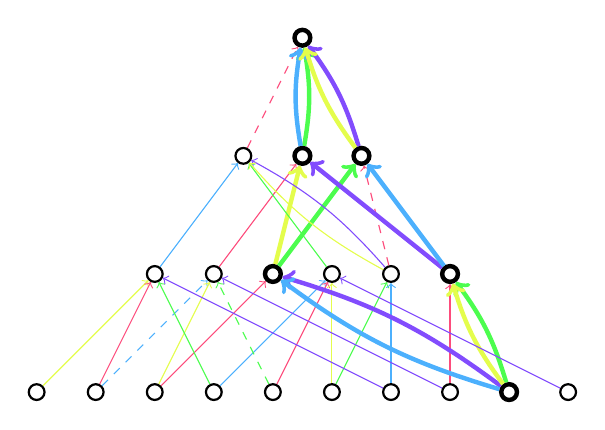
\begin{tikzpicture}[scale=1,bend angle=10]
\newcommand{\xspace}{1}
\newcommand{\yspace}{1}
\tikzstyle{vertex}=[draw,thick,circle,minimum size=2mm,inner sep=0pt]
\tikzstyle{edge}=[->]
\tikzstyle{onesided}=[edge,dashed]
\tikzstyle{bothsided}=[edge]
\tikzstyle{unhighlighted}=[]
\tikzstyle{highlighted}=[ultra thick]
\definecolor{s1color}{RGB}{130,76,253}
\definecolor{s2color}{RGB}{76,253,78}
\definecolor{s3color}{RGB}{253,76,124}
\definecolor{s4color}{RGB}{76,176,253}
\definecolor{s5color}{RGB}{228,253,76}
\tikzstyle{s1}=[s1color]
\tikzstyle{s2}=[s2color]
\tikzstyle{s3}=[s3color]
\tikzstyle{s4}=[s4color]
\tikzstyle{s5}=[s5color]
\node[vertex,unhighlighted] (56) at (\xspace*-3.375,\yspace*9) {};
\node[vertex,unhighlighted] (57) at (\xspace*-2.625,\yspace*9) {};
\node[vertex,unhighlighted] (58) at (\xspace*-1.875,\yspace*9) {};
\node[vertex,unhighlighted] (59) at (\xspace*-1.125,\yspace*9) {};
\node[vertex,unhighlighted] (60) at (\xspace*-0.375,\yspace*9) {};
\node[vertex,unhighlighted] (61) at (\xspace*0.375,\yspace*9) {};
\node[vertex,unhighlighted] (62) at (\xspace*1.125,\yspace*9) {};
\node[vertex,unhighlighted] (63) at (\xspace*1.875,\yspace*9) {};
\node[vertex,highlighted] (64) at (\xspace*2.625,\yspace*9) {};
\node[vertex,unhighlighted] (65) at (\xspace*3.375,\yspace*9) {};
\node[vertex,unhighlighted] (66) at (\xspace*-1.875,\yspace*10.5) {};
\node[vertex,unhighlighted] (67) at (\xspace*-1.125,\yspace*10.5) {};
\node[vertex,highlighted] (68) at (\xspace*-0.375,\yspace*10.5) {};
\node[vertex,unhighlighted] (69) at (\xspace*0.375,\yspace*10.5) {};
\node[vertex,unhighlighted] (70) at (\xspace*1.125,\yspace*10.5) {};
\node[vertex,highlighted] (71) at (\xspace*1.875,\yspace*10.5) {};
\node[vertex,unhighlighted] (72) at (\xspace*-0.75,\yspace*12) {};
\node[vertex,highlighted] (73) at (\xspace*0,\yspace*12) {};
\node[vertex,highlighted] (74) at (\xspace*0.75,\yspace*12) {};
\node[vertex,highlighted] (75) at (\xspace*0,\yspace*13.5) {};
\draw[s5,bothsided,unhighlighted] (56) edge (66);
\draw[s3,bothsided,unhighlighted] (57) edge (66);
\draw[s4,onesided,unhighlighted] (57) edge (67);
\draw[s5,bothsided,unhighlighted] (58) edge (67);
\draw[s3,bothsided,unhighlighted] (58) edge (68);
\draw[s2,bothsided,unhighlighted] (59) edge (66);
\draw[s4,bothsided,unhighlighted] (59) edge (69);
\draw[s2,onesided,unhighlighted] (60) edge (67);
\draw[s3,bothsided,unhighlighted] (60) edge (69);
\draw[s5,bothsided,unhighlighted] (61) edge (69);
\draw[s2,bothsided,unhighlighted] (61) edge (70);
\draw[s1,bothsided,unhighlighted] (62) edge (66);
\draw[s4,bothsided,unhighlighted] (62) edge (70);
\draw[s1,bothsided,unhighlighted] (63) edge (67);
\draw[s3,bothsided,unhighlighted] (63) edge (71);
\draw[s1,bothsided,highlighted,bend right] (64) edge (68);
\draw[s4,bothsided,highlighted,bend left] (64) edge (68);
\draw[s2,bothsided,highlighted,bend right] (64) edge (71);
\draw[s5,bothsided,highlighted,bend left] (64) edge (71);
\draw[s1,bothsided,unhighlighted] (65) edge (69);
\draw[s4,bothsided,unhighlighted] (66) edge (72);
\draw[s3,bothsided,unhighlighted] (67) edge (73);
\draw[s5,bothsided,highlighted] (68) edge (73);
\draw[s2,bothsided,highlighted] (68) edge (74);
\draw[s2,bothsided,unhighlighted] (69) edge (72);
\draw[s1,bothsided,unhighlighted,bend right] (70) edge (72);
\draw[s5,bothsided,unhighlighted,bend left] (70) edge (72);
\draw[s3,onesided,unhighlighted] (70) edge (74);
\draw[s1,bothsided,highlighted] (71) edge (73);
\draw[s4,bothsided,highlighted] (71) edge (74);
\draw[s3,onesided,unhighlighted] (72) edge (75);
\draw[s2,bothsided,highlighted,bend right] (73) edge (75);
\draw[s4,bothsided,highlighted,bend left] (73) edge (75);
\draw[s1,bothsided,highlighted,bend right] (74) edge (75);
\draw[s5,bothsided,highlighted,bend left] (74) edge (75);
\end{tikzpicture}
%		\caption{Upper end of Hasse diagram of $Wk(A_5,\id)$}
%		\label{fig:main-thesis-weakend-hypothesis-counterexample}
%	\end{figure}
%\end{exam}

A hypothesis, that is much stronger than \ref{ques:main}, reads $wC_I \cap wC_J = wC_{I \cap J}$. If this would be true, \ref{ques:main} could be concluded immediately. Unfortunately it proves to be false. Again, double-edges yield a simple counterexample.

\begin{exam}
	\typedlabel{exam:cap-of-residuums}
	Let $w \in \ti{\theta}$ and $s,t$ two distinct generators with $w \ul s = w \ul t = v$. Then $wC_{\{s\}} \cap wC_{\{t\}} = \{w,v\} \neq \{w\} = wC_{\emptyset} = wC_{\{s\} \cap \{t\}}$.
\end{exam}

\begin{prop}
	\typedlabel{prop:s1-in-s2-main-special-case}
	Let $S_1,S_2,S_3,S_{12},S_{23},S_{31},T$ like in \ref{ques:main}. Suppose one set of $S_1,S_2,S_3$ is contained by another. Then
	$$ \forall \ 1 \leq i < j \leq 3 : v \in w C_{S_{ij}} \quad \Rightarrow \quad v \in w C_T. $$

	\begin{proof}
		Let $S_1 \subset S_2$. Then we have $S_{12} = S_1$. By this we get the identity
		$$ T = S_1 \cap S_2 \cap S_3 = S_{12} \cap S_3 = S_1 \cap S_3. $$
		Hence $v \in w C_T = w C_{S_{31}}$.
	\end{proof}
\end{prop}